\chapter{Architecture/Model}
\label{cha:architectureAndModel}
This chapter contains the architecture and model of the system, which tools and methods that has been used, how they all connect together to run the experiments and produce the result.
An overview of the system is presented in chapter \ref{sec:overview}. A description of the robot is presented in section \ref{sec:robot}. How the robots calculate where to move is explained in section \ref{sec:robotcontroller}. The brief explanation of the simulator is found in section \ref{sec:simulator}, and the biggest difference between the physical experiment and the simulator is shown and compared in section \ref{sec:vs}. The math used to plot the graph are shown in section \ref{sec:makeres}.

Throughout this chapter the word "Boids" will solely refer to the Boids on the simulator, while entity or entities refer to both the physical robots and the Boids.

\begin{figure}[h]
\begin{center}
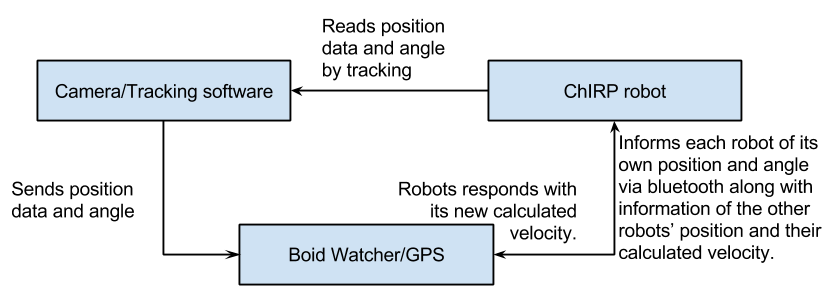
\includegraphics[width=\linewidth]{figs/system_overview}
\end{center}
\caption[System overview]{Overview of the components of the system}
\label{fig:overview}
\end{figure}

\section{System overview}
\label{sec:overview}

The system used in this experiment consists of three primary components as illustrated in figure \ref{fig:overview}: the camera which is used by the tracking software, the "Boid-watcher" which is a centralized computer that acts as a GPS and the ChIRP robots.
The camera tracking software tracks each robot's position and its angle, which is sent to the Boid-watcher. The Boid-watcher then forward this information to the robots via the Bluetooth serial port.

The Boid watcher does not only work as a GPS, but it is also a communication bridge between the robots, it provides information about the position and velocity of each robot to all the other robots. The robots are not able to connect to the other robots directly, that is why the they need to pass information to the other robots through the watcher software via Bluetooth.

Even if it is possible for one computer to run both the camera tracking and the watcher software, two separate computers were used in this setup. The camera tracking software being run on a stationary desktop computer, and the camera is attached to a pole above a sandbox where the robots roam around. The camera is connected to the stationary desktop. 

In this experiment, the watcher software runs on a laptop with a built-in Bluetooth adapter. The watcher software needs to communicate with all the robots simultaneously and that requires processing powers.
The desktop computer was not able to run both the camera tracking software and the watcher software at the same time while sending Bluetooth data to all four of the robots. When it tried to run both, it was not able to read the data from the camera fast enough and thus the tracking software would crash. The Bluetooth connection between the computer and the robots might not always be stable, if the connection were to be unstable at times, a reboot of the robot or/and a reconnection of the Bluetooth connection would usually fix the problem.

The camera tracks the robots using image recognition, it recognizes the robots by the two circular post-it notes that are placed on top of each robot. 
To filter out all the noise from the surrounding area and remove the colors that are irrelevant to track, the camera tracking software needs to have a threshold for what it considers to be red and what it considers to be green. This is specified in a configuration file that the camera tracking software loaded whenever it was launched. An example of the configuration file can be seen in the appendix on section \ref{app:opencvcfg}. As seen in the example, each color is defined by six boundaries, a minimum value, and a maximum value for the hue-saturation-value. If a color seen by the camera is inside this boundary it will be considered as the color it is looking for.\clearpage

\begin{figure}[H]
    \centering
    \begin{subfigure}[b]{0.55\textwidth}
        \centering
        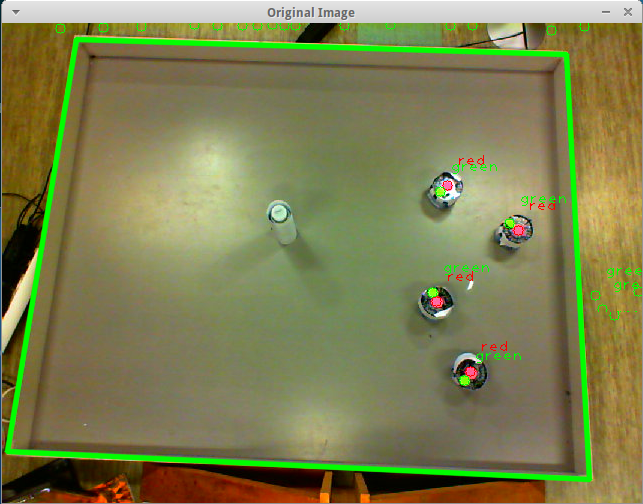
\includegraphics[width=\textwidth]{figs/camOrig}
        \caption{Original image}
        \label{fig:camorig}
    \end{subfigure}
    \hfill
    \begin{subfigure}[b]{0.4\textwidth}
        \centering
        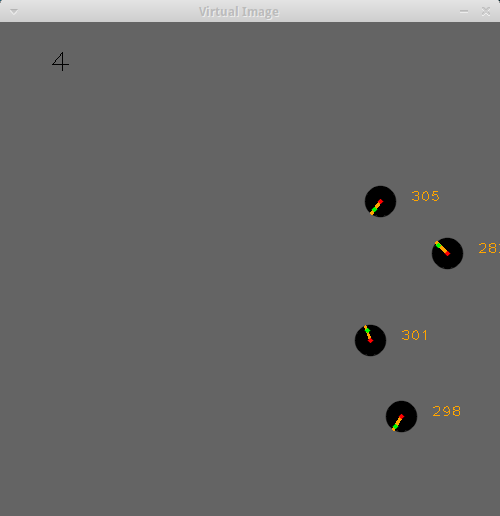
\includegraphics[width=\textwidth]{figs/camVirt}
        \caption{Virtual image}
        \label{fig:camvirt}
    \end{subfigure}
    \caption[Camera tracking software]{Images from the camera tracking software}
    \label{fig:cam}
\end{figure}

The camera might detect red or green colors that do not belong to the robots, for example when the sun shines into the room, the green part of the floor around the sandbox might be detected as "green" by the camera tracking software. This is not a problem for the camera tracking software because this green floor is outside of the predefined box and the tracker only tracks colors that are inside of this predefined box, which the user has to specify when starting up the software. This predefined tracking are is the green outline in figure \ref{fig:camorig}. Any robots found outside of this green boundary box are not tracked, only the robots inside this predefined area will be tracked and have a legal position value and an angle. That is why we need a sandbox to contain the robots so they do not wander off outside the range of the green boundary box where they are not tracked anymore. Only the position and the angle of the tracked robots will be sent to the Boid watcher software over UDP.

Detecting red or green color inside the sandbox that does not belong to the robots imposes a bigger problem than detecting these colors outside the box. This might happen if there is a green shaded shadow or a reflection of an object reflects onto the sandboxes' surface.
If the software detects green or red color that do not belong to the robot, it will simply ignore these colors if the green and the red color are far apart from each other, because the camera tracking software does not do anything unless both these colors are paired. If these "noise" colors do disrupt the movement or angle of the robots, then a recalibration needs to be done to filter out the colors and make the tracking more precise.

\section{Robots}
\label{sec:robot}
\begin{figure}[H]
    \centering
    \begin{subfigure}[b]{0.3\textwidth}
        \centering
        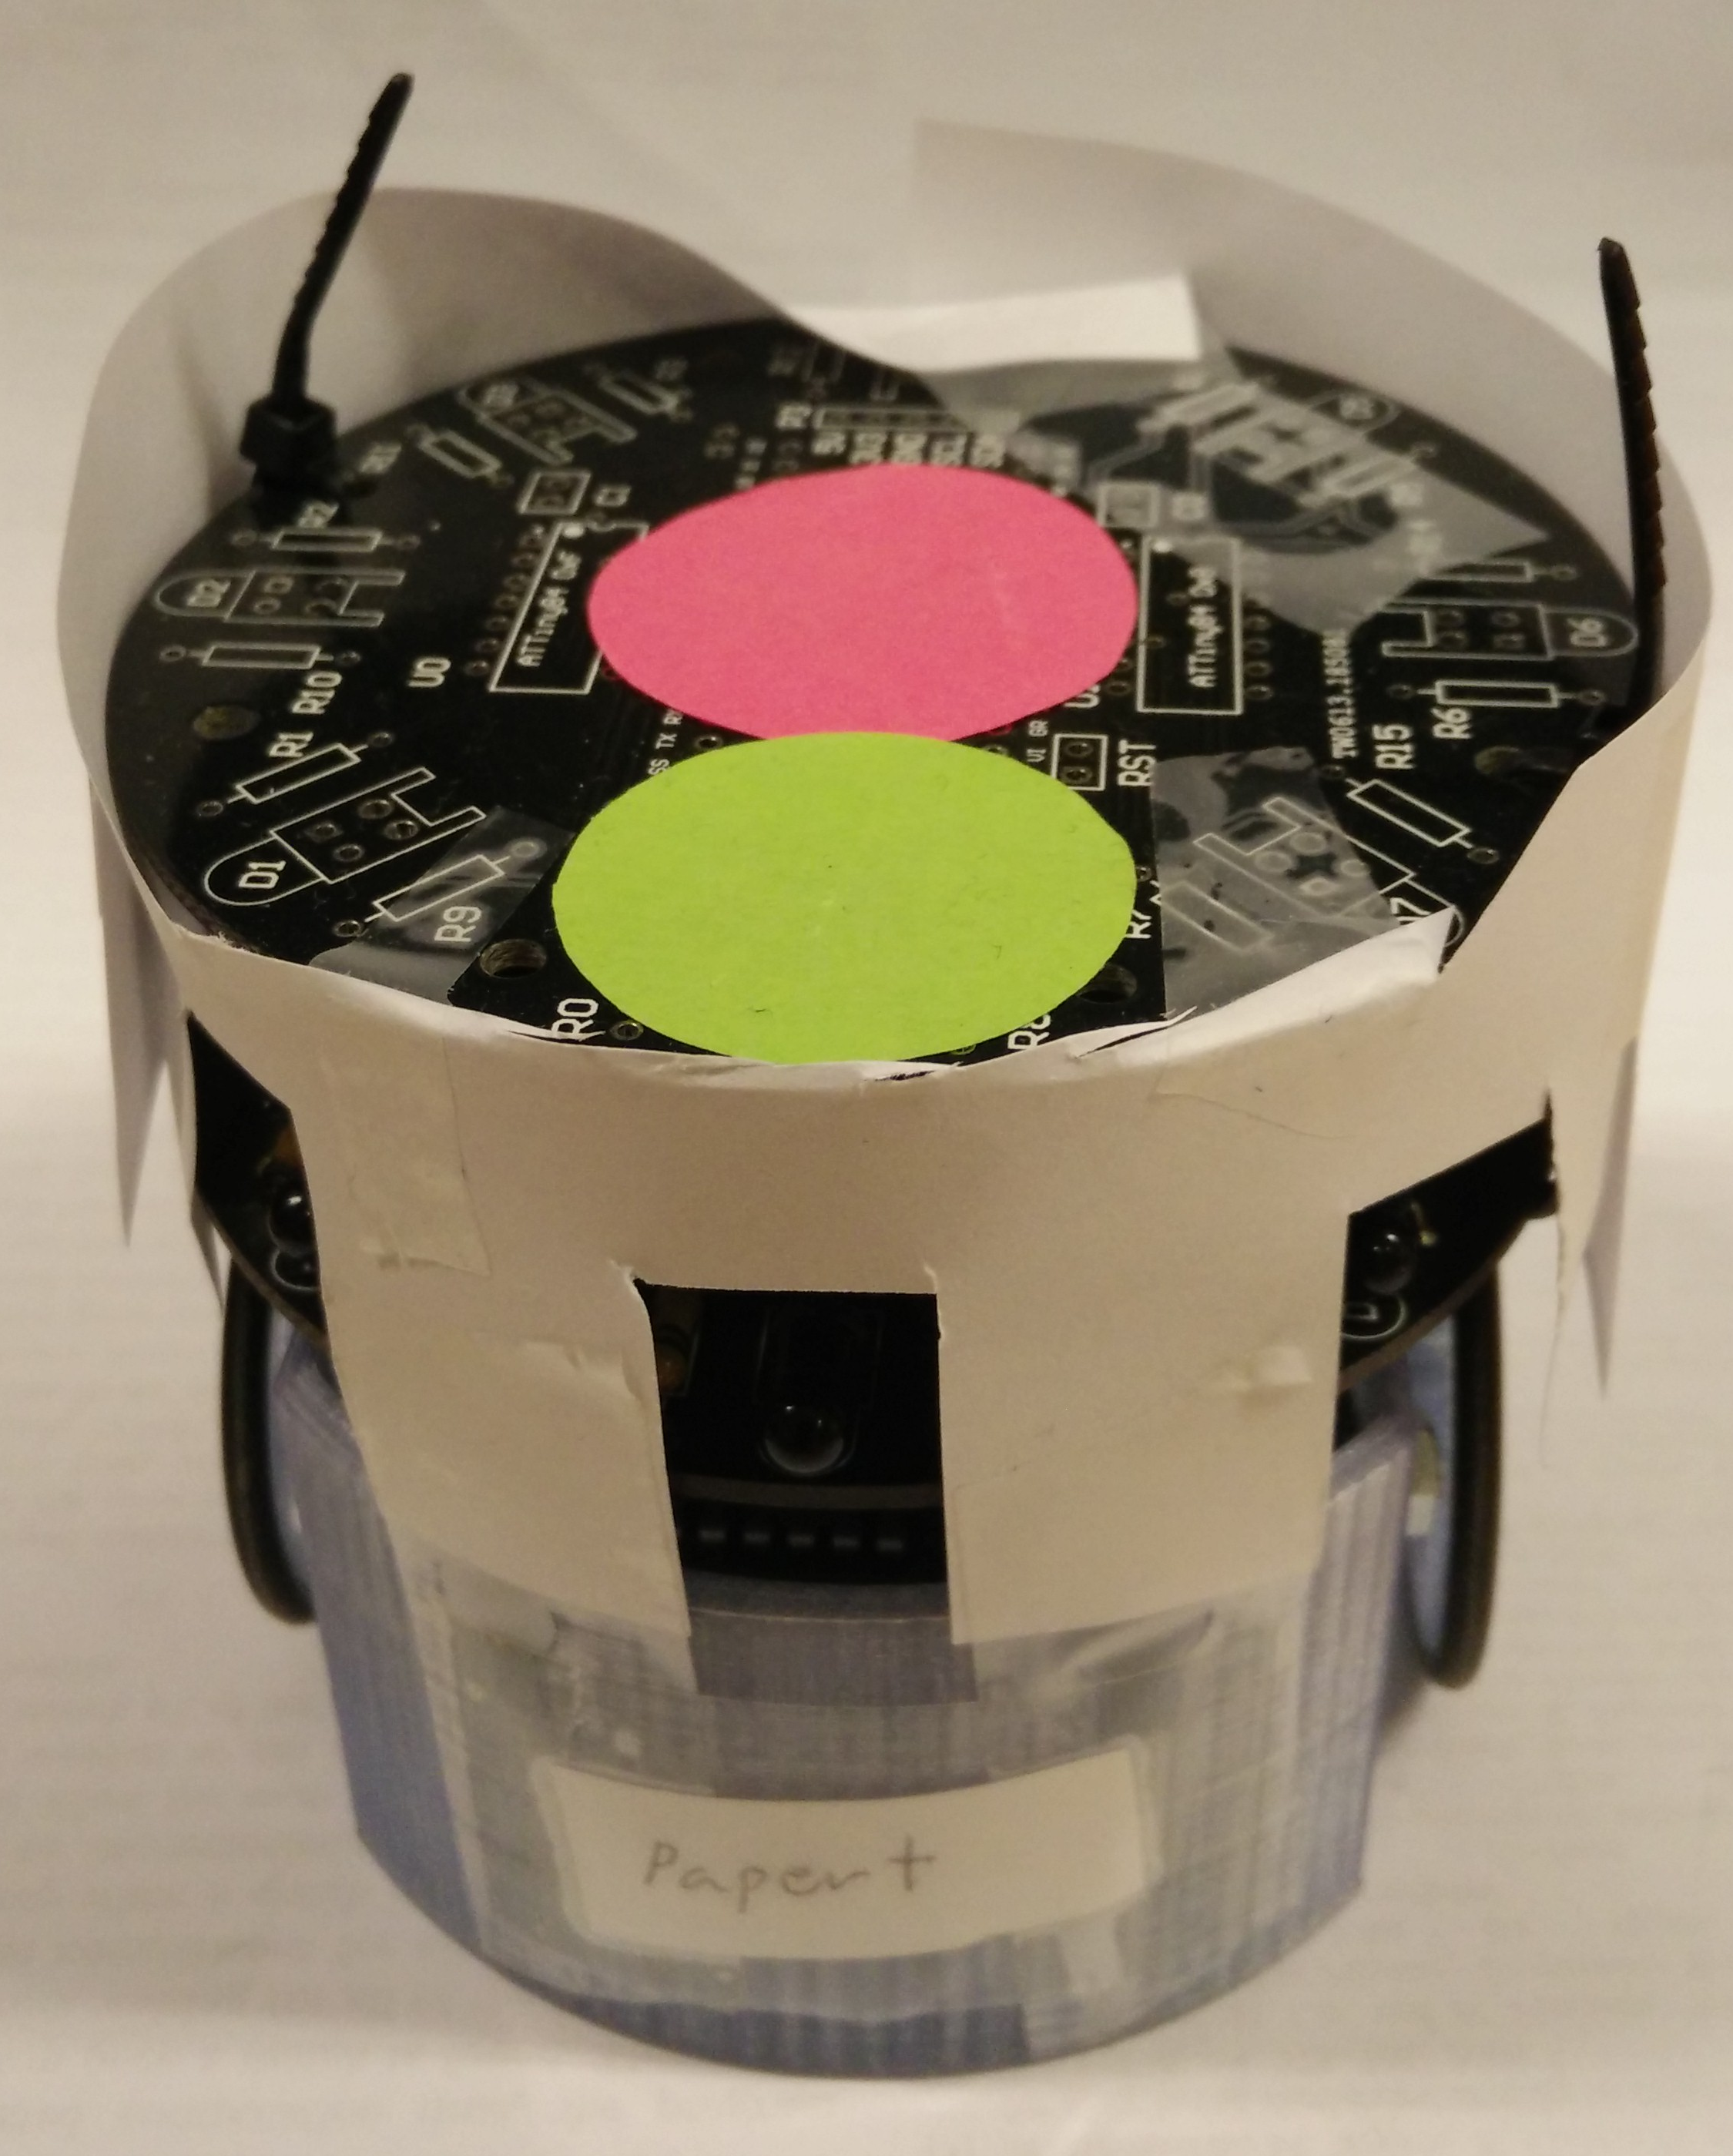
\includegraphics[width=\textwidth]{figs/robot1}
        \caption{The robot used in the experiment}
        \label{fig:robot0}
    \end{subfigure}
    \hfill
    \begin{subfigure}[b]{0.3\textwidth}
        \centering
        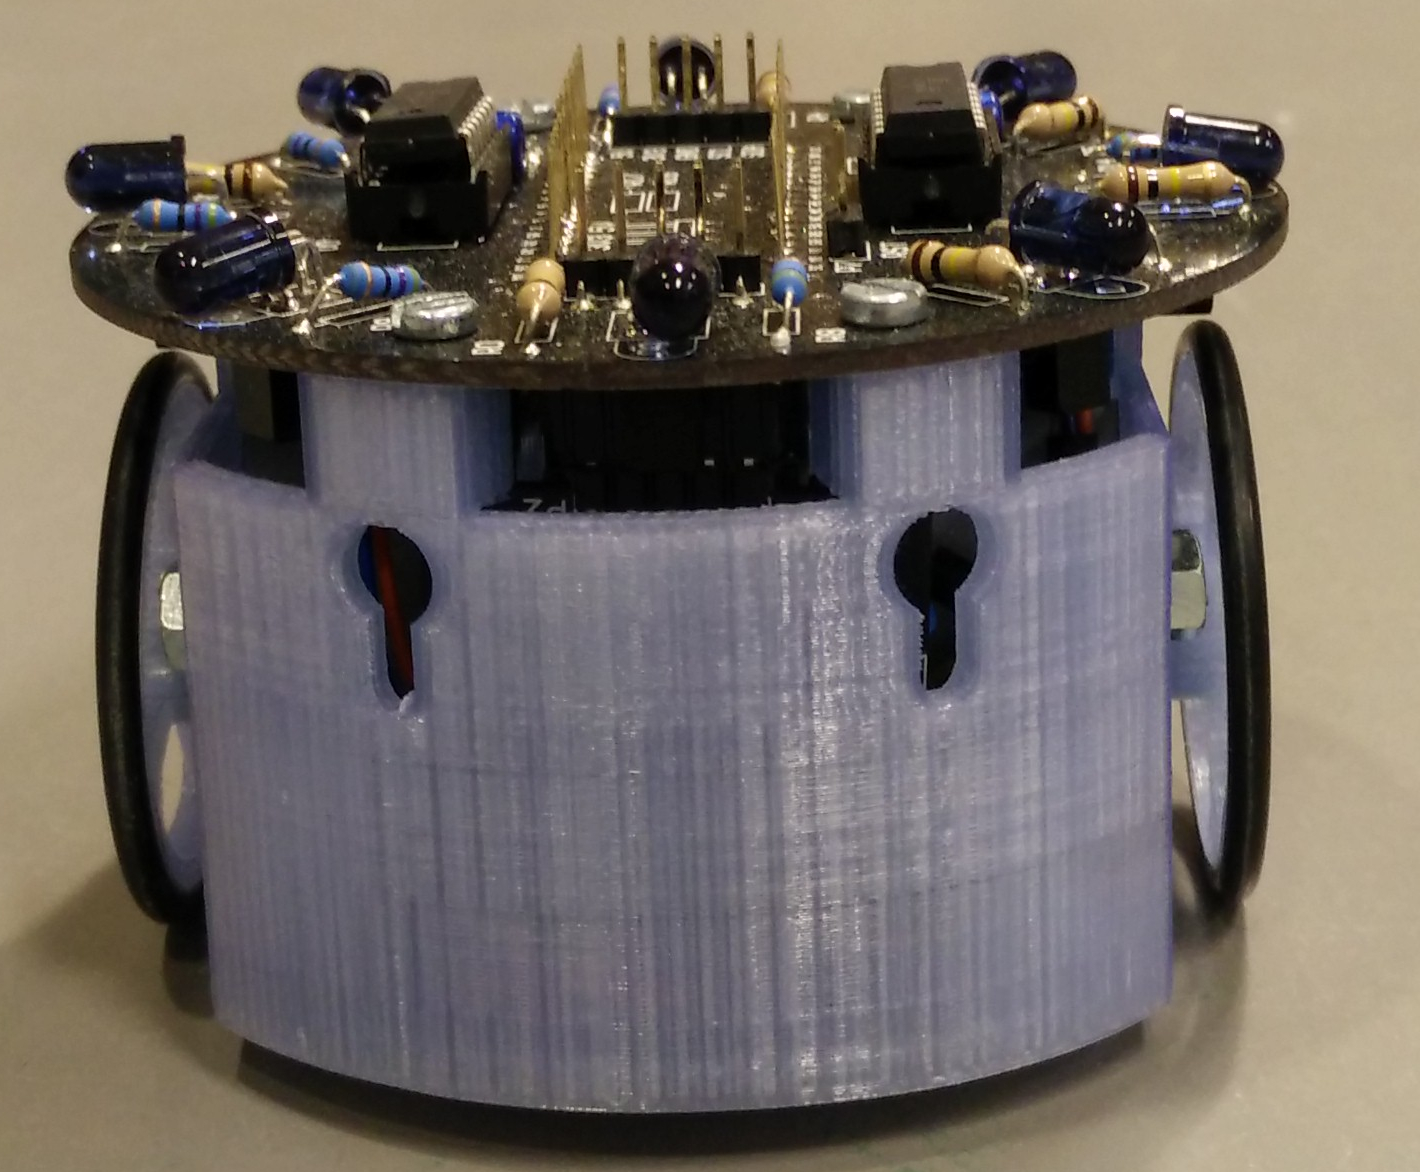
\includegraphics[width=\textwidth]{figs/robot2}
        \caption{Standard ChIRP robot}
        \label{fig:robot1}
    \end{subfigure}
    \hfill
    \begin{subfigure}[b]{0.3\textwidth}
        \centering
        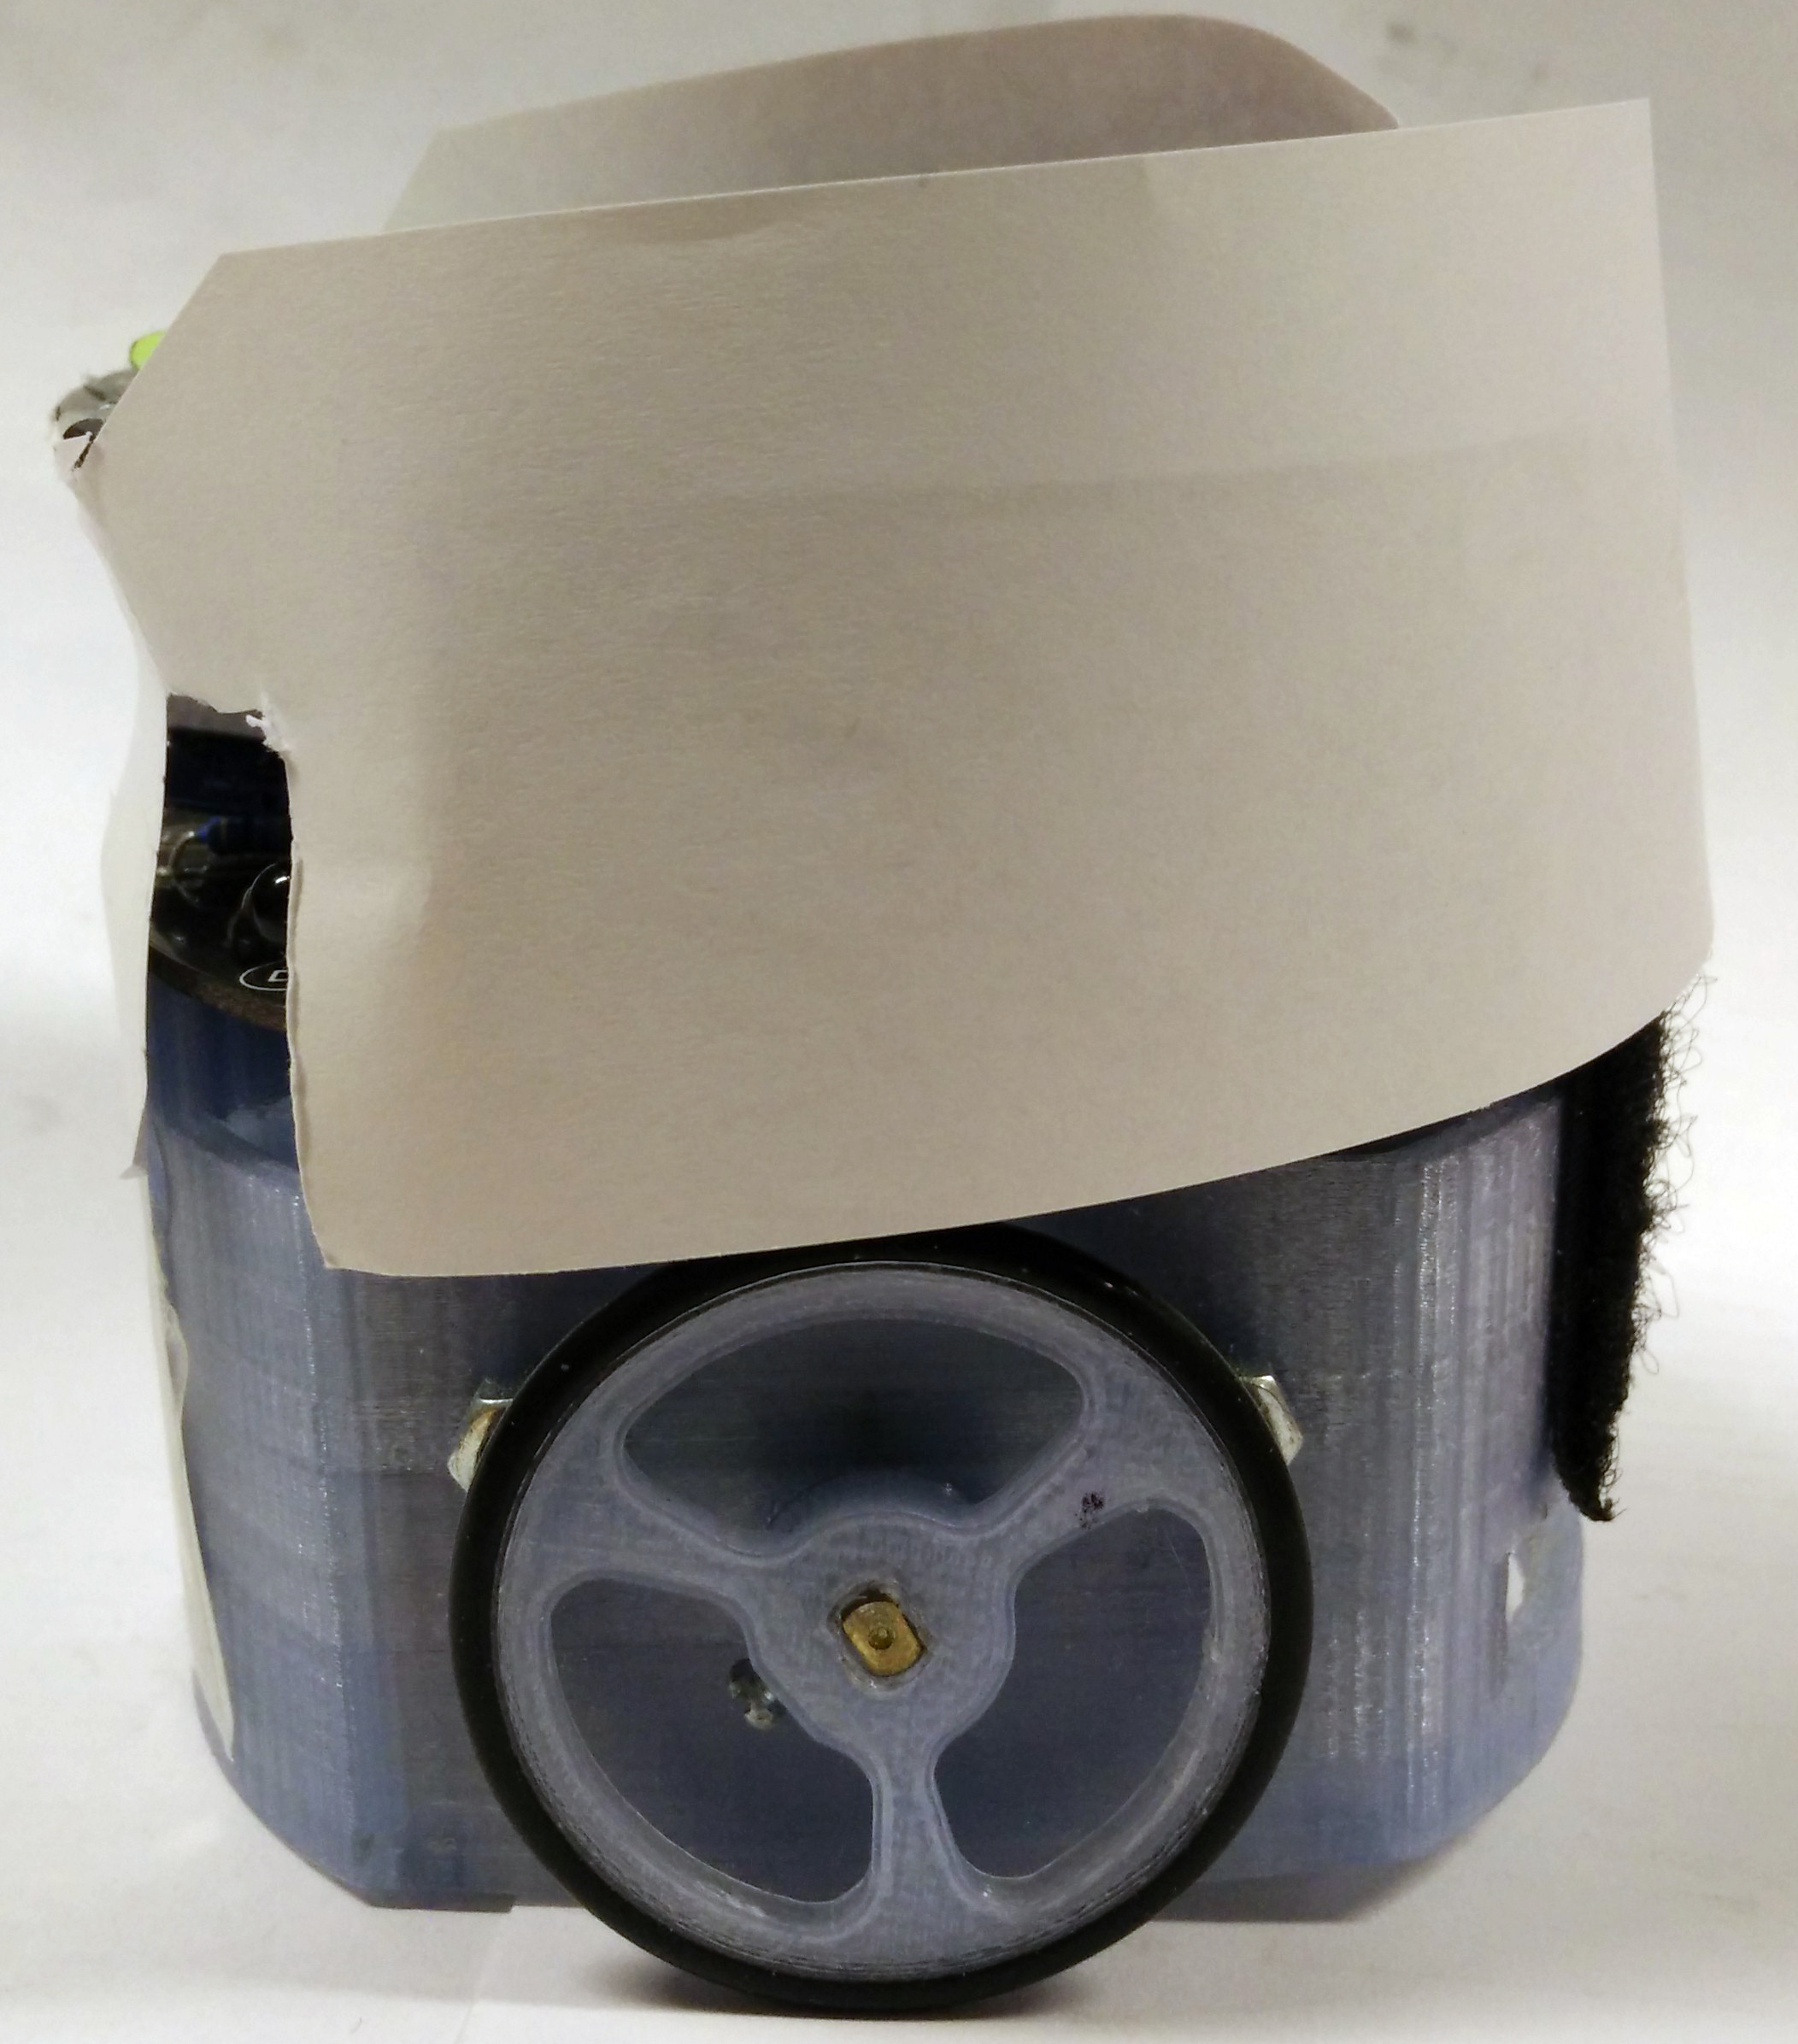
\includegraphics[width=\textwidth]{figs/side}
        \caption{ChIRP seen from the side}
        \label{fig:robot3}
    \end{subfigure}
    \caption[ChIRP robot]{ChIRP robot seen from various angles}
    \label{fig:robot}
\end{figure}



The robot swarm consists of four ChIRP robots. The ChIRP robot is a circular shaped robot with differential wheel. A differential wheeled robot is a robot with two separate driven wheels on each side, which it can use to move itself. If it wants to change its direction it can vary the relative speed of each wheel or motor. For instance if the right wheel moves faster than the left one, the robot will turn to its left.
The advantage of differential wheel is that an additional steering motor is not required for the robot to move around. Usually a caster or additional wheels are added to balance a differential wheeled robot, but the ChIRP robot does not have anything of the sort. Whenever it is moving, the back or the front of the robot is scraping against the floor depending on if it has a backward or forward momentum. Scraping against the floor does not affect the movement of the ChIRP robot, it was designed this way. The robots have a max speed of approximately 13 cm/s, in this experiment the velocity of the robot will not exceed 7.8 cm/s. 

Each robot is equipped with eight infrared LED lights and receivers used for measuring distance. Infrared light are emitted from the LEDs, reflected on a surface and received in the infrared receiver. For the robot to know how far from an obstacle it is, it measures the amount of infrared it receives. The higher the amount, the closer to the object it is. This method of measuring distances works very well for bright or colored surfaces, dark surfaces on the other hand do cause problems because the infrared light is not reflected so well.

The distance sensors are spaced evenly around the robot, where one of the sensors are pointing directly in front of the robot. This sensor can be used to detect whether there is an obstacle directly in front of it. For this experiment, only the three sensors in front are used. Because the robots only moves forward, so it only needs to determine whether there is an obstacle directly in front of it. The two other distance sensors are also needed, because using only the one in front is not sufficient to determine if the robot is going to crash into an object. The other sensors on the side or the back of the robot is not used because the robot does not move in that direction.
So it does not matter if there is an obstacle behind or on the side of the robot.

Each of the ChIRP robots is equipped with a Bluetooth module, which it uses to communicate with the watcher computer wirelessly. 
The robots are very hollow on top as seen in figure \ref{fig:robot1} and the distance sensors have difficulties sensing other robots due to this hollowness. To counteract the hollowness, a white paper strip was taped around the robots. This makes it easier for the robot to detect the other robots nearby because the paper will reflect the infrared light that the robot uses to determine the distance. To be sure that the robot would be able to detect the obstacles placed in the sandbox, the obstacle would have a white paper wrapped around it to reflect the infrared light. The obstacle used for this experiment consist of a bottle filled with water. The water inside the bottle is used to make it heavier, so it does not fall over if a robot were to crash into it. And the paper around the bottle is there to reflect the infrared light that the robot uses for measuring distances.

The camera tracking software uses image recognition to track the robots. That is why each robot needs to have a red and a green post-it note on top of it. The red one determines where in the sandbox the robot is located, and the green one is used to decide which way it is pointing and to determine the angle of the robots.

\section{Robot controller}
\label{sec:robotcontroller}
This section will go through the controller of the robot, how they work and what steps the robot takes to execute its action.

The robots are implemented using the idea of a hybrid robot control architecture as explained in section \ref{sec:hybrid}. The distances sensors are the reactive layers which will be used to guide the robots away from crashing into obstacles, walls or other robots. The deliberative layer will be the code that processes the data sent from the watcher software on the computer, it calculates where the robot should be heading. The deliberative layer are usually slow, but the robots in this experiment are aided by the centralized computer, it does not need to use a lot of its processing power to map the environment. The robot already knows that they are roaming inside a sandbox, and they already knows the size of this sandbox.
The executive layer would be the code running on the robot that decides what the robot is doing, whether that is reading the sensors and avoiding obstacles or moving towards the planned destination for flocking.

When the robot is turned on and a Bluetooth device is paired with its Bluetooth module, the robot will stand still and wait. The robot is waiting for a command or data from the watcher software. A human can send commands to manually control the robot if needed, this can for example be used for leader following as explained in section \ref{boids:behaviors}. 

If the watcher sends data to the robot, it will start to calculate where it should move based on the data it received. 
%When the robot have received all the data from the watcher software, it will start to calculate each vector and it will calculate a final acceleration vector that will determine where it should move. 
The robot takes into consideration the position and the velocity of all the other robots. The positions of the other robots are used to determine the sum of the cohesion vector and the separation vector. The velocity of the other robots are used to determine which way they are pointing, and this is used to find the alignment vector.

A fourth behavior was added for this experiment, which is called the "away from wall" behavior. As the name implies, this is a vector that will lead the robot away from the wall of the sandbox if the robot is too near the wall. After calculating each of these vectors, they are multiplied with a weight depending on how much that specific behavior should impact the movement of the robot. For example, the separation vector should have a higher impact on the movement of the robot because it needs to avoid the other robots when it is too close to one. 

Cohesion vector, on the other hand, does not need to affect the robot as much, it is mostly there to guide the robot into the flock. Therefore, the separation vector is multiplied with a higher number than the other ones.


The equation for how the final acceleration vector which decides the direction the robot is going to move is expressed as: 
\begin{equation}
\label{eq:vecsum}
\vec{A} = \Sigma_{i=1}^{N_b}(W_i\vec{B_i})
\end{equation}

where:
\\
$\vec{A}$ = the acceleration vector
\\
$B_i$ = the behavior $i$, for example $B_1$ could be cohesion behavior, $B_2$ alignment behavior etc.
\\
$W_i$ = the weight for the behavior $B_i$\\
$N_b$ = the number of behaviors\\

The neighborhood distances used on the physical robots are the following ones:
\begin{description}
\item[cohesion distance] = 800 px
\item[alignment distance] = 200 px
\item[separation distance] = 150 px
\item[away from wall distance] = same as alignment
\item[obstacle distance] = same as separation
\end{description}

Each of these behaviors, which is denoted by $B_i$ in equation \ref{eq:vecsum}, and the following weights $W_i$ have been used:
\begin{description}
\item[cohesion] vector is multiplied by 2
\item[alignment] vector is multiplied by 2
\item[away from wall] vector is multiplied by 1
\item[avoid obstacles] does not exist
\item[separation] vector is multiplied by 4
\end{description}

After calculating the acceleration vector, it will add it to its velocity vector, then use the arctangent function to calculate which direction the robot will turn to. The robot calculates the new direction it needs to face by using the following equations:
\begin{equation}
\label{eq:veladdacc}
\vec{V}_{new} = \vec{V}_{old} + \vec{A}
\end{equation}
\begin{equation}
\label{eq:atan2}
R_{goal} = atan2(\vec{V}_y, \vec{V}_x)
\end{equation}
\begin{equation}
\label{eq:angletoturn}
D_{turn} = (R_{goal} - R_{current})* \frac{180}{\pi}
\end{equation}
\begin{equation}
\label{eq:accelreset}
\vec{A} = [0,0]^T
\end{equation}

where:
\\
$\vec{V}_{old}$ = previous velocity of the robot
\\
$\vec{V}_{new}$ = new velocity of the robot, the length of $\vec{V}_{new}$ is capped between -40 and 40 or using mathematic notation: $ |\vec{V}_{new}| \epsilon [-40,40]$.
\\
$R_{goal}$ = the angle the robot will be facing after it has turned around, measured in radians, $R_{goal} \epsilon [-\pi,\pi]$
\\
$R_{current}$ = the angle the robot is currently facing, measured in radians,
$R_{current} \epsilon [-\pi,\pi]$
\\
$D_{turn}$ = the angle the robot needs to turn to face the correct direction, measured in degrees. $D_{turn} \epsilon [-180,180]$
\\


The robot needs to know how much it is going to move in the x-direction and how much it will move in the y-direction as shown in equation \ref{eq:veladdacc}.
Then by calculating the arctangent of $V_x$ and $V_y$, it finds out which angle it needs to face to be able to move in the direction of $\vec{V}_{new}$. When the robot has calculated which direction it wants to go, it calculates $D_{turn}$ by using the formula in equation \ref{eq:angletoturn}. $D_{turn}$ is the amount of degrees the robot needs to turn to face the right direction. The velocity $\vec{V}_{new}$ is only used to determine which direction the robot should be facing, it is not used for determine the velocity of the robot. The velocity of a robot is calculated by calculating how much the robot has been moving since the last time step, or by finding out how much the position of the robot has changed since the last time step: 
\begin{equation}
\label{eq:calcrobvel}
V_{robot} = \Delta P = P_{new} - P_{old}
\end{equation}

When the robot has received the data from the watcher, it will first check measure the distance in front of it, to check if there is an obstacle in front of it. If there is on, it will turn away from the obstacle, and wait for new data from the watcher. If the path is clear, it will do the calculation shown in equation \ref{eq:vecsum} trough \ref{eq:accelreset}. Then the robot will turn $D_{turn}$ degrees so it will face the correct direction.

The robot will then measure the distances once again, in case it has turned towards an obstacle. If there is no obstacle in front of it, it will move forward while waiting for new data from the watcher software. If the robot did find an obstacle in front of it, it will turn 90\textdegree to either the right or the left randomly. The robot will stop after turning and wait for new data from the watcher software. 
\begin{figure}[h!]
\begin{center}
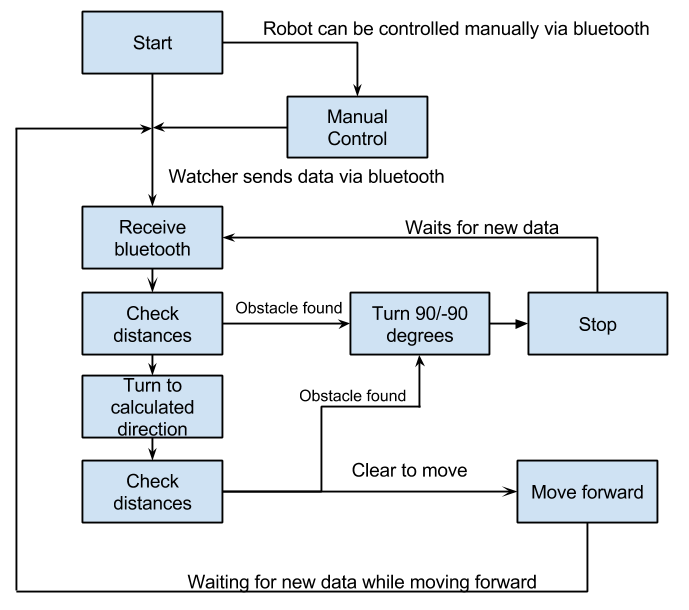
\includegraphics[width=0.8\linewidth]{figs/robotschema}
\end{center}
\caption[Robot flowchart]{Flowchart of the robot's behavior}
\label{fig:robotschema}
\end{figure}
\clearpage

\section{Simulator}
\label{sec:simulator}
A simulator was created where the Boids was implemented solely in software, and rendered on screen, that is no physical robots were used in the simulator. The reason to use a simulator was to see how the Boids were supposed to behave and have a working example to compare with. A screenshot of the simulator is shown in figure \ref{fig:simulatordistances}.

A typical Boids simulator usually have a wraparound space. If one of the Boids goes outside the window, it will "teleport" to the other side of the window. For example if one of the Boids flies too far to the right and hits the right border of the window, it will loop around and end up on the left side of the window. This is how the typical Boids algorithm usually works on a simulator. But physical robots can not loop around the stage like the Boids on the simulator can. That is why the simulator used in this project stops the Boids from moving beyond the walls of the window.

The same "away from wall" behavior is also implemented in the simulator, so the Boids do not move into the wall aimlessly.

For each frame, the Boids will update it velocity by calculating a vector for each behavior, and then these vectors are added to the acceleration vector by using the formula found in equation \ref{eq:vecsum}. The acceleration vector is then added to the velocity vector, and the velocity is capped off if the length of the vector exceeds the maximum allowed speed. If there is no velocity cap, the Boids' velocity would increase towards infinity. The velocity then decides where the Boids are going to move.
The procedure to calculate the velocity vector of the simulated Boids are the same as the one the robots are using; in equation \ref{eq:veladdacc}. 

After calculating the $\vec{V}_{new}$, it needs to cap the max velocity. If the velocity is not capped, the speed of Boids would increase and they would move outside the window. As for the robots, the Boids velocity vector is kept between -40 and 40:  $|\vec{V}_{new}| \epsilon [-40,40]$.
The Boids do not need to calculate which way it needs to turn to move in the direction, because it is able to move in all 360\textdegree\ directions without the need to turn. The robot had to turn because it could not move sideways, it could only move either forward or backward.

The Boids simply moves by adding the velocity vector to their position:
\begin{equation}
\label{eq:posadd}
P_{new} = P_{old} + \vec{V}
\end{equation}

where:\\
$P_{old}$ = old position of the Boid\\
$P_{new}$ = new position of the Boid\\

Before the next time step, the acceleration has to be reset to a null vector for it to work as shown in equation \ref{eq:accelreset}.

The Boids in the simulator do not have any form of rotation, the angle seen on screen are calculated by taking the arctangent of the velocity vector. That is why the Boids in the simulator do not need to rotate; they change their direction instantly by changing their velocity.

In the simulator, there is no need for any type of sensors. Each Boid has access to the location of all the obstacles and all the other entities.

%Each Boid in the simulator are rendered as a circle, so they are as similar as the real ChIRP robot, however, there are some big differences between the real ChIRP robot and the Boids in the simulator. 

In the simulator, the following parameters have been used:
\begin{description}
\item[cohesion distance] = 250 px
\item[alignment distance] = 175 px
\item[separation distance] = 120 px
\item[away from wall distance] = same as alignment
\item[obstacle distance] = same as separation
\end{description}
These distances are used by the Boids to determine how near it has to be before it should calculate the vector. For example if the Boid is in the middle of the screen, that means that it is not near a wall, then the "away from wall" function will return the null vector because it does not need the Boid to steer away from the wall.


These behavior distances is the furthest distance that is needed before activating this behavior, for instance, a Boid that have three neighbors, where one of them is 100 px away, the second one is 150 px away while the third one is 300 px away. The first Boid will be taken into consideration when calculating all of the three behaviors; cohesion, alignment and separation because it is very close. The second Boids will not have any influence on the separation behavior, but it will influence the alignment and cohesion vector. The third one is too far away, and will be ignored when calculating the three behaviors. These distances are illustrated in figure \ref{fig:simulatordistances}.
The Boids in the simulator has a velocity cap of 40 px per frame, moving faster than 40 px would make the Boids move too fast, and it would be hard to clearly see the details of the movements. 

Each vector from each behavior is multiplied with a factor that determines how much impact that vector will have on the final acceleration vector.
The list provided below is the weight multiplied by the behavior vector. Or the $W_i$ found in equation \ref{eq:vecsum}.

\begin{description}
\item[cohesion] vector is multiplied by 2
\item[alignment] vector is multiplied by 2
\item[away from wall] vector is multiplied by 2
\item[avoid obstacles] vector is multiplied by 3
\item[separation] vector is multiplied by 3
\end{description}

%Visually, the Boids are circles on the screen, but all the Boids in the simulator are in fact just a mathematical point with a position. 

\section{Differences between the physical experiment and simulator}
\label{sec:vs}
Although the robot's behavior are trying to mimic the behaviors found on the simulated Boids, some major differences will still be imminent. This section will explain the biggest differences between the physical experiment and the simulator. 

The physical robots are trying to mimic the behavior of the Boids created in the simulator. However, a physical robot is different than the Boids created in the simulator by nature. As discussed in section \ref{sec:robot}, the robots are a type of differential wheeled robots, which means that it can only move forward or backwards, turn on the spot or move and turn at the same time. It can not move sideways.

The Boids in simulator software did not have any direction, they were able to move freely in all 360\textdegree direction. Which means that if a Boid in the simulator were to move in one direction, it could change its momentum and move the other direction without having to stop and turn to that direction. The robot, on the other hand, would need to turn 180\textdegree before moving forward. The robot is able to reverse its motor to drive backward, but these robot are not allowed to move backward, and thus have to turn around to move in another direction.

In the simulator, each Boid will know exactly where everything is placed. That is, each Boid knows where all the other Boids are, including itself. It also knows where all the obstacles are. The Boids will have real time access to everything that can be seen on screen. Every Boid will update its perception every frame, that is approximately 60 times every second.

The robots, on the other hand, will receive data from the watcher about all the other robots. But due to inaccuracies from the camera and the image processed, the robots only knows vaguely where in the sandbox it is located, and where the others are. The time it takes for a robot to receive new information from the watcher takes roughly one second from the last time it received data from the watcher. If the robots are moving between the time it receives data, it will not know where it is before it receives new data from the watcher software. The camera tracking software is able to see all the robots due to the two post-it notes on top, but obstacles found in the sandbox do not contain any color or anything that the camera can track. Obstacles are therefore ignored by the camera tracker software because it does not support tracking of anything other than the robots. That is why the robots need to use their distance sensors in the front to detect the obstacles.

The biggest most visual difference between the physical experiment in the sandbox and the simulated Boids is the size and speed of the entities. The size of the simulator is 1024 px times 1024 px. While the sandbox is 151.6 cm wide and 123.9 cm long, which corresponds to 800x652 px in the watcher software. The Boids on the simulator moves quite fast and can use the extra space to move around, while the robots are confined inside the sandbox. The biggest reason to use 800x652 px for the watcher software is because the behavior neighborhood distances works well for this size.

\begin{figure}[h]
\begin{center}
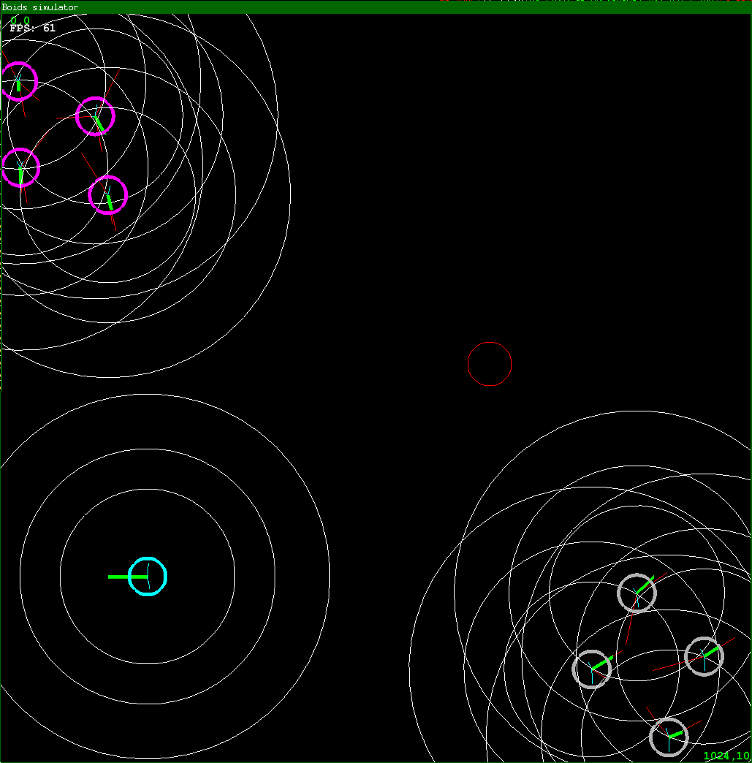
\includegraphics[width=0.8\linewidth]{figs/simulator}
\end{center}
\caption[Simulator distances]{Simulated Boids with neighborhood distances visualized}
\label{fig:simulatordistances}
\end{figure}



As it will be explained later in section \ref{sec:experimentalSetup}, the parameters for the simulated Boids and the physical robots are a bit different.
The figure \ref{fig:simulatordistances} shows the approximate distances for each behavior, the inner thick colored ring is the outline of the Boids. The inner thin white ring, illustrates the separation distance, the robot do not try to separate itself from the other robots if they are outside this ring.

The red lines in the figure, are the vectors from each behavior before it is multiplied with the weight. The thickest green line indicates which way the Boids are moving, the longer the line, the faster the Boids are moving.

The second most outer ring indicates the alignment neighborhood, if there is another Boid inside this ring, then both of them will try to align and move in the same direction.

The outer circle is the cohesion distance, the Boids outside of this box will not attract each other.


In the figure \ref{fig:simulatordistances}, three types of Boids "family" exist, each one has their own color. Boids will flock together and align themselves only if they have the same color, that is the light gray Boids will flock together with the other light gray Boids. The magenta Boids will only flock together with the other magenta Boids.

When running the simulation for the experiment, all four of the Boids were the same color, therefore just one flock of Boids would emerge instead of forming multiple flocks. The current implementation of the Boids algorithm on the robots does not support multiple groups of Boids. There is no point in implementing this functionality when there are only four robots running at the same time, because it will be very hard to distinguish the difference between a family group flock or if there is just a robot astray from the flock.

\begin{figure}[h]
\begin{center}
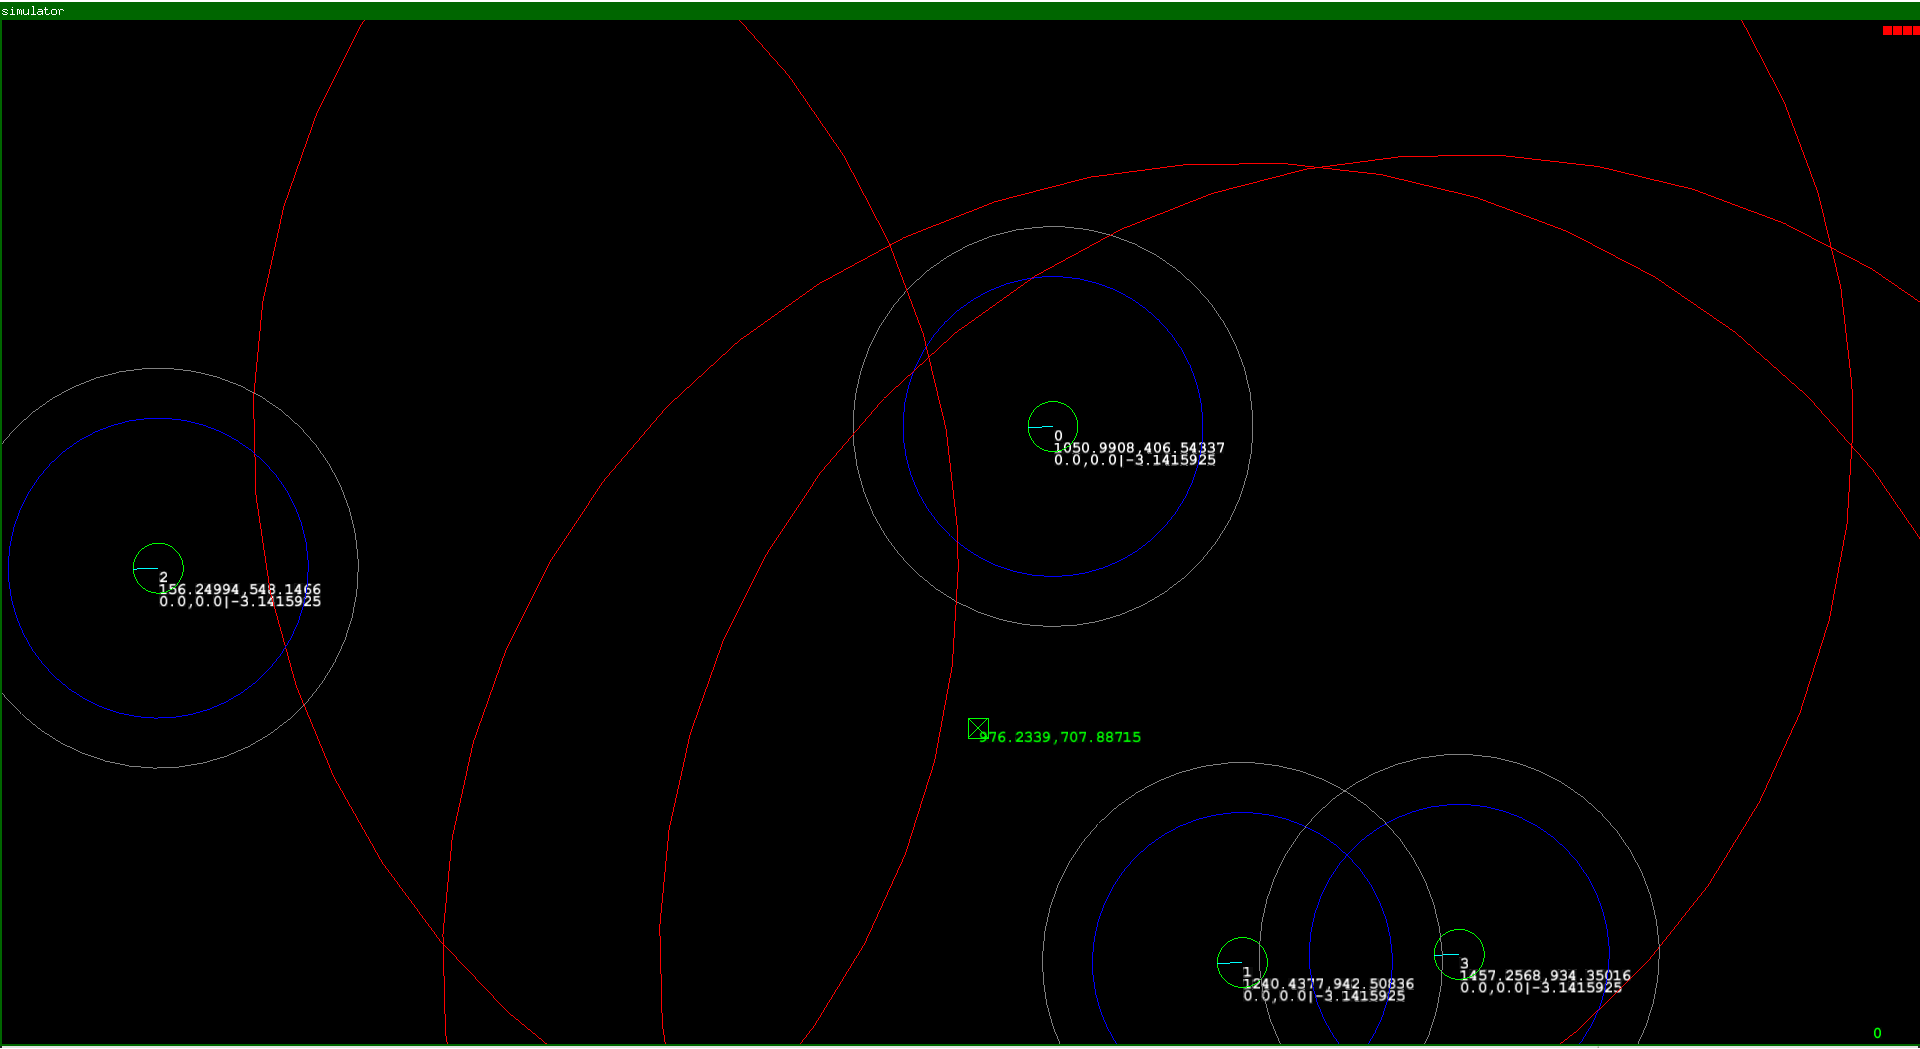
\includegraphics[width=1.1\linewidth]{figs/wathcer}
\end{center}
\caption[Watcher software]{Watcher software with neighborhood distances visualized}
\label{fig:watcher}
\end{figure}

Figure \ref{fig:watcher} illustrates the distances that the robots use. The exact numbers can be found in section \ref{sec:experimentalSetup}. The distances have been colored for convenience because it is hard to see which ring represents which behavior. As in the simulator, the most inner ring, which is green in this figure represents the outline of the robot. The figure shown is not the same size as the watcher software that is used to run the experiments, the resolution of the watcher software on the figure has a resolution of 1024x1920 px which is a lot bigger than the resolution on the watcher software used in the experiment. This is to make it easier to see and distinguish the distances.

The next ring, which is illustrated with a blue color, represents the separation distance. And the gray ring shows the alignment neighborhood distance. These two distances are the same in the simulator and on the robot.

The biggest red ring is the one that is the most different from the simulator's.
The reason the cohesion distance is so large is mainly to force the robots to flock together even when they are far apart. The distance almost covers the whole sandbox, that way the robots will try to flock from almost anywhere in the sandbox.


Information about each robot is also provided by the numbers next to each robot.
The first row shows us the ID of the robot, and the serial port that belongs to that robot if there is a Bluetooth connection and it is assigned.
The second row shows us the position of the robot, while the third one shows velocity and the angle of the robot.

The upper right red squares indicate whether the Bluetooth connection is still functional or if the Bluetooth have timed out. The squares in the figure are all red because this is just a debug run where there is no Bluetooth connection.

Robots will be pushed away if a different robot moves onto it. Two robots can not occupy the same space at the same time. Simulated Boids can overlap without affecting each other.
To summarize the difference between the robots and the simulated Boids, a list of the parameters will be shown here:
\begin{table}[h]
\begin{center}
\begin{tabular}{|l|l|l|}
\hline
\multicolumn{3}{|c|}{Neighborhood distances} \\ \hline
Behavior          & Simulator    & Robots    \\ \hline
Cohesion          & 250 px          & 800 px       \\ \hline
Alignment         & 175 px          & 200 px      \\ \hline
Separation        & 120 px          & 150 px      \\ \hline
Away from wall    & 175 px          & 200 px      \\ \hline
Obstacle          & 120 px          & 150 px      \\ \hline
\end{tabular}
\caption[Neighborhood distance comparison]{Table comparing neighborhood distances between robots and simulated Boids}
\end{center}
\label{tab:dists}
\end{table}

\begin{table}[h]
\begin{center}

\begin{tabular}{|l|l|l|}
\hline
\multicolumn{3}{|c|}{Vector weights} \\ \hline
Behavior        & Simulator & Robots \\ \hline
Cohesion        & 2x        & 2x     \\ \hline
Alignment       & 2x        & 2x     \\ \hline
Separation      & 3x        & 4x     \\ \hline
Away from wall  & 2x        & 1x     \\ \hline
Obstacle        & 3x        & Does not exist   \\ \hline
\end{tabular}
\end{center}
\caption[Weights comparison]{Table comparing weights applied to behaviors between robots and simulated Boids}
\label{tab:weights}
\end{table}

The reason the cohesion distance for the physical robot are so different than the one in the simulator is because the robots are slow to flock together and they might get stuck at a corner when the sensors, so a big cohesion distance makes the robots flock together faster. If the robots' cohesion distance were to be the same as the cohesion distance for the simulated Boids, they might stay too long in one place, and the robots might not flock. As shown in later sections, the robots flocks with an average distance of 200 px, therefore the cohesion distance has to be sufficient larger than 200 px for it to be effective. 

The Boids in the simulator do not need a cohesion distance of 800, because they wander a lot around even if there are no neighboring Boids around them. When they have wandered around for a while, they will eventually find another Boid that is near enough and they will start to flock together.

The weights on the behavior vectors for the robots are a little bit different than the one found in the simulator. The robot's behavior weight are kept as close to the Boids as possible, but some weights had to be tweaked for the experiments.

As seen from the table \ref{tab:weights}, the avoid obstacle vector does not exist for the robots because the watcher and the camera tracking software can not find nor distinguish obstacles from the surroundings. This feature is not implemented in the camera tracking software. The robot needs to know the size of the sandbox beforehand because the camera or the watcher software do not provide this information to the robot. To compensate for the lack of obstacle information, the robot uses their distance sensors to find out where the obstacle are located and avoids them.

As seen in the list above, the two vectors that have the highest influence on the robot is the separation and the obstacle avoidance behavior. These two behaviors needs to influence the robot a lot more than the other behaviors because they are only activated when the robot is very close to another robot or an obstacle.

\section{How results are made}
\label{sec:makeres}
This section will go through the process of how the results found in section \ref{sec:results} are made.

The results are created by writing to a text file in the form of a .csv file, which can be open directly by spreadsheet software. A csv file is simply a text file with comma separated values, a row in the csv file would correspond to a row in the spreadsheet, and a column in the spreadsheet software is separated by a comma in the csv file. The distances between the entities, the difference between their angle and the velocity are the features that the watcher software will be graphing.

The watcher software has no way to find the actual velocity of the robots because the wheels still move when the robot is turning on the same spot. We want to find out if the position of each robot has changed over a given time interval.
The way the watcher software calculates the velocity of each robot is to save the old position of the robot, then compare it with the new position and see how far off it is.
The formula used to find the mean velocity value of all the robots at a time step is defined as:
\begin{equation}
\label{eq:muvel}
\mu_{velocity} = \frac{1}{N} \Sigma_{i=1}^N |P_{i_{new}} - P_{i_{old}}|
\end{equation}

where:
\\
$p_{i_{new}}$ = the new updated position of robot $i$
\\
$p_{i_{old}}$ = the old position of robot $i$ from last time step
\\
$N$ = number of robots used, in this experiment $N = 4$ 
\\
$\mu_{velocity}$ = the mean of the velocities in that time step

The average distance seen in section \ref{sec:results} are calculated the same way for both the physical experiment and in the simulator. Each entity's position is found and compared with the position of all the other entities. The length of the distance between each of them are used to find the average and the standard deviation.
The formula to find 

\begin{equation}
\mu_{distances} = \frac{1}{ {N \choose R}} \Sigma_1^{N \choose R} | P_i - P_j |
\end{equation}

where:
\\
$P_i$ = the position of robot i, and $i \neq j$
\\
$P_j$ = the position of robot j, and $i \neq j$
\\
$N$ = the number of robots or Boids used
\\
$R$ = the amount of entities that are being compared each time, in this experiment we only measures the distance between two entities at the same time, therefore $R = 2$.
\\
$N \choose R$ = the combination operator, this corresponds to $ \frac{N!}{R! (N-K)!}$
\\
$\mu_{distances}$ = the mean of the compared distances in that time step
\\

The same procedure was applied for the angle of each entity: 
\begin{equation}
\mu_{angles} = \frac{1}{ {N \choose R}} \Sigma_1^{N \choose R} | A_i - A_j |
\end{equation}
where:
\\
$A_i$ = the angle of robot x, and $i \neq j$
\\
$A_j$ = the angle of robot y, and $i \neq j$
\\
$\mu_{angles}$ = the mean of the compared angles in that time step.
\\

To find the standard deviation of the velocity, the formula in equation \ref{eq:sd} was used, but a modification was done for the standard deviation of the distances and angles as seen in equation \ref{eq:sd2} because we had $ {N \choose R}$ number of distances and angles. The reason for $ {N \choose R}$ number of distances is because this is the number of comparisons between each robot. For these experiments, $N = 4$, and $R = 2$ because we use 4 robots and there is a comparison between two robots at the same time.


\begin{equation}
\label{eq:sd}
\sigma =  \sqrt{\frac{1}{N}\Sigma(X-\mu)^2}
\end{equation}

\begin{equation}
\label{eq:sd2}
\sigma =  \sqrt{\frac{1}{{N \choose R}}\Sigma(X-\mu)^2}
\end{equation}




